% options:
% thesis=B bachelor's thesis
% thesis=M master's thesis
% czech thesis in Czech language
% slovak thesis in Slovak language
% english thesis in English language
% hidelinks remove colour boxes around hyperlinks

\documentclass[thesis=M,czech]{FITthesis}[2012/06/26]
\usepackage[section]{placeins}
\usepackage[utf8]{inputenc} % LaTeX source encoded as UTF-8

\usepackage{graphicx} %graphics files inclusion
% \usepackage{amsmath} %advanced maths
% \usepackage{amssymb} %additional math symbols

\usepackage{dirtree} %directory tree visualisation


% % list of acronyms
% \usepackage[acronym,nonumberlist,toc,numberedsection=autolabel]{glossaries}
% \iflanguage{czech}{\renewcommand*{\acronymname}{Seznam pou{\v z}it{\' y}ch zkratek}}{}
% \makeglossaries

\newcommand{\tg}{\mathop{\mathrm{tg}}} %cesky tangens
\newcommand{\cotg}{\mathop{\mathrm{cotg}}} %cesky cotangens
\usepackage[within=none]{caption}
\renewcommand\thetable{\Roman{table}}
% % % % % % % % % % % % % % % % % % % % % % % % % % % % % % 
% ODTUD DAL VSE ZMENTE
% % % % % % % % % % % % % % % % % % % % % % % % % % % % % % 

\department{Katedra počítačových systémů}
\title{Analýza síťového provozu s pomocí komunikačních map}
\authorGN{Tomáš} %(křestní) jméno (jména) autora
\authorFN{Vicher} %příjmení autora
\authorWithDegrees{Bc. Tomáš Vicher} %jméno autora včetně současných akademických titulů
\supervisor{Ing. Tomáš Čejka}
\acknowledgements{Rád bych poděkoval vedoucímu práce Ing. Tomáši Čejkovi za rady a čas, které mi věnoval. Dále bych rád poděkoval rodině a přítelkyni za podoporu při práci.}
\abstractCS{Podstatou a cílem diplomové práce je navrhnout metodu zpracování informací o síťových tocích k vygenerování a udržování grafu komunikace mezi jednotlivými uzly sítě, popřípadě agregovaných uzlů (podsítí). Navrhnout využití pro vzniklé struktury ke sledování vývoje provozu, případně k detekci neobvyklých jevů na síti. Výsledkem práce je detekční metoda implementovaná jako modul do systému NEMEA.
Součástí práce je také rešerše možností monitorování sítě, útoků na síť a statistických metod pro analýzu síťových toků.}
\abstractEN{The aim of the master thesis is to design method of processing information about network flow to generate and preserve graph of communication between network nodes or agregated nodes (subnetworks). The purpose is to design and implement usage for the formed structures to monitor network traffic and detect anomaly. The result of the master thesis is the detection method implemented as a module to the NEMEA system.}
\placeForDeclarationOfAuthenticity{V~Praze}
\declarationOfAuthenticityOption{4} %volba Prohlášení (číslo 1-6)
\keywordsCS{síťová analýza, síťový tok, Holt-Wintersova metoda, python, monitorování, graf, simulace}
\keywordsEN{network analysis, network flow, Holt-Winters method, python, monitoring, graph, simulation}
\usepackage{chngcntr}
\begin{document}

\counterwithout{figure}{chapter}
\renewcommand{\thefigure}{\arabic{figure}}
% \newacronym{CVUT}{{\v C}VUT}{{\v C}esk{\' e} vysok{\' e} u{\v c}en{\' i} technick{\' e} v Praze}
% \newacronym{FIT}{FIT}{Fakulta informa{\v c}n{\' i}ch technologi{\' i}}

\begin{introduction}
\section{Motivace}
Počet počítačů a dalších zařízeních spojených sítí se stále zvyšuje jak v domácnostech, tak ve firmách spolu s celosvětovým trendem zlepšující se dostupnosti internetového připojení \cite{itgrowing}. Reakcí na tyto změny je potřeba vývoje a zlepšování síťové bezpečnosti se kterou je spojeno monitorování sítí. S tím přichází problém kdy je zvyšována bezpečnost na úkor snižování soukromí. V této práci je monitorování zpracováno s účelem zvýšení bezpečnosti, ale jeho zneužití může sloužit k škodlivým účelům. Mezi využitím k zvýšení bezpečnosti Z motivace pro monitorování sítě lze zmínit například:
\begin{itemize}
	\item Zvýšení bezpečnosti pro citlivá a důležitá data přenášená po síti a uchovávaná v zařízeních připojených k síti.
	\item Optimalizace využití a hardwaru. 
\end{itemize}
Kvůli stále rostoucímu trendu kyberkriminality je důležité nebrat monitorování jako okrajovou záležitost v IT.\cite{cybercrime}
\par
Tato práce se zabývá monitorováním sítí pomocí síťových toků a jejím účelem je vytvořit nástroj, který pomůže IT administrátorům monitorovat síť a rozpoznat případné nečekané události v síti. 
Pro zařazení monitorování do komplexnějšího přehledu bezpečnosti v IT je uveden obrázek s hierarchií zabezpečení.\ref{img:security_hierarchy}. Politika zabezpečení v IT začíná od správy zařízení a inventarizace, pokračuje správou a údržbou software. Další vrstvou je kontrola nad identitou uživatelů, zaměstnanců,... Na předchozí vrstvy zabezpečení navazuje řízení přístupu ke zdrojům a informacím. Na vrcholu této bezpečnostní pyramidy se nachází detekční metody - téma na které je zaměřena tato diplomová práce.\cite{networkhierarchy}

	\begin{figure}[!htbp]\centering
		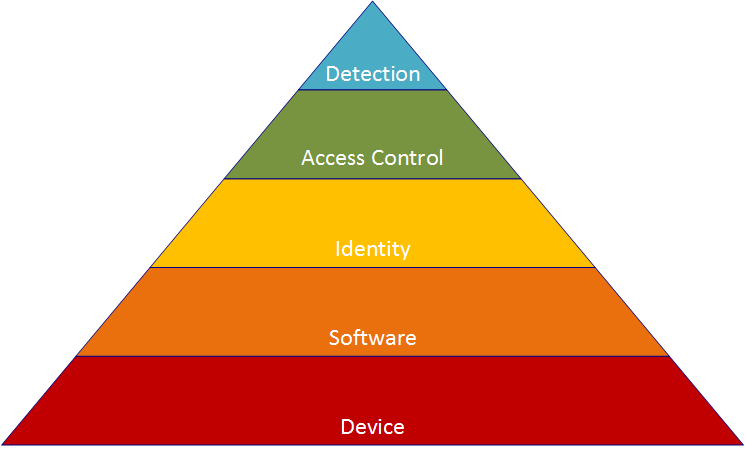
\includegraphics[width=0.8\textwidth]{security_hierarchy.png}
		\caption[Hierarchie zabezpečení v IT. Zdroj: \cite{networkhierarchy}]{Hierarchie zabezpečení v IT. Zdroj: \cite{networkhierarchy}}
		\label{img:security_hierarchy}
	\end{figure}
	
\section{Struktura práce}
V první části je vypracována rešerše zpracování síťového provozu, anomálií a statistických metod. Ve druhé části je s informacemi získanými rešerší navrženo řešení pro monitorování síťového provozu s využitím síťových toků. Třetí část popisuje použité nástroje a implementaci navrženého řešení jako modul do systému Nemea\footnote{Nemea je systém fungující na základě modulů umožňující real-time monitorování sítě. Další informace a zdrojové kódy jsou na adrese \url{https://github.com/CESNET/Nemea}}. Ve čtvrté části jsou uvedeny testy s výsledky testování implementovaného modulu. V závěrečné části je uvedena diskuze, zhodnocení splněných cílů práce a možnosti budoucího rozšíření.
\end{introduction}

\chapter{Specifikace cílů}
Kapitola popisuje rozbor zadání, tedy rozbor cílů práce. 
\section{Rozbor zadání}
\subsubsection*{Nastudujte způsob monitorování síťového provozu na základě sledování síťových toků}
Úkolem je vyhledat a nastudovat informace o síťových tocích. Nastudovat možnosti monitorování sítě na základě sledování síťových toků. S tímto úkolem souvisí zpracování informací o dostupných technologiích pro práci s toky, způsobů síťových útoků a statistických metod pro zpracování a vyhodnocování dat.  
\subsubsection*{Navrhněte metodu zpracování informací o síťových tocích k vygenerování a udržování grafu komunikace mezi jednotlivými uzly sítě popř. agregovaných uzlů (podsítí)}
Na základě nastudovaných informací z předchozího bodu je úkolem navrhnout metodu, jakou lze zpracovat a udržovat informace přijaté ze síťových toků v podobě grafu.
\subsubsection*{Navrhněte využití vzniklých grafových struktur ke sledování vývoje provozu na síti, případně k detekci	neobvyklých jevů na síti}
S využitím informací z prvního bodu zadání je úkolem navrhnout způsob využití dat připravených v grafové struktuře za účelem vyhodnocování provozu v síti. Při sledování provozu detekovat neobvyklý stav ukazující na anomálii v provozu. 

\subsubsection*{Navrženou detekční metodu implementujte jako modul do systému Nemea}
Z návrhu vzniklého v předchozích bodech je úkolem implementovat aplikaci, která bude odpovídat specifikacím systému Nemea pro použití jako modul a integraci do Nemea systému.
\subsubsection*{Otestujte tento mechanismus za pomoci simulace příp. s použitím reálného provozu z počítačové sítě}
Úkolem je implementovanou aplikaci otestovat na datech z reálného nebo simulovaného síťového provozu a otestovat implementované monitorovací a detekční metody. 

\chapter{Rešerše}
V této kapitole jsou uvedeny způsoby monitorování a detekce změn v síti, útoků na síť a statistických metod. V první sekci kapitoly jsou uvedeny možnosti monitorování změny v síti. V dalších sekcích rešerše jsou popsány metody monitorování síťového provozu na úrovni paketů a síťových toků. V souvislosti s monitorováním toků je v rešerši zahrnuta sekce věnující se systému Nemea pro který byl v rámci práce navrhnut a implementován modul. Dále se rešerše zaměřuje na útoky na síť, které lze monitorovat a detekovat s využitím analýzy síťových toků. V závěrečné části uvádím rešerši statistických metod pro použití k detekci anomálií v síťovém provozu.

\section{Zpracování síťového provozu}
Monitorování síťového provozu lze podle způsobu zpracování síťových dat rozdělit na dvě skupiny. Analýza paketů, při které je vyhodnocování anomálií prováděno pomocí signatur a analýzu chování sítě, která probíhá na základě zpracování síťových toků.

\subsection{Analýza paketů pomocí signatur}
Jednou z možností rozpoznání anomálií v síťovém provozu je detekce na základě signatur na úrovní jednotlivých paketů. Tento způsob využívají IDS systémy\footnote{Intrusion detection system}. Signatury jsou vzory, které jsou vyhledávány v síťovém provozu. Mohou být vytvořeny podle návrhu systému ve kterém jsou použity. Záleží na konkrétním IDS jakou možnost tvorby nebo modifikace signatur uživatelům poskytuje, ale základním předpokladem pro úspěšnou detekci pomocí signatur je výběr IDS nebo vytvoření správných signatur pro problém, na který se má detekční systém zaměřovat. Níže je uvedeno příkladem několik vybraných signatur s popisem situace, kterou s nimi lze monitorovat. \cite{signatures}
\begin{itemize}
	\item Detekce připojení IP adresy, která je rezervovaná pro jiné zařízení. Lze odhalit kontrolou parametru zdrojové adresy v hlavičce paketu.
	\item Detekce paketů se špatně nastavenými flagy. Lze odhalit porovnáním s dobrými/špatnými vzorovými kombinacemi.
	\item Identifikace nežádoucího doručeného emailu. Lze rozpoznat porovnáním obsahu předmětu, nebo jiných částí zprávy se vzorem.
	\item Pokus o DNS buffer overflow může být odhalen rozparsováním DNS dotazu a kontrolou délky obsahu.
	\item DOS útok který je realizován pomocí velkého množství stejných dotazů nebo obsahujících charakteristickou část lze odhalit pomocí jejich počítání.
\end{itemize}
Z principu používání signatur vychází nevýhoda v nízké účinnosti odhalování zero-day útoků\footnote{Zero-day je typ útoků, které jsou realizovány v den, kdy byly vytvořeny.}. V bezpečnostních systémech založených na principu signatur v té době ještě neexistují signatury, se kterými by je mohl systém odhalit. V softwaru na který je útok cílen obvykle existuje chyba, která nebyla ještě opravena.\cite{zeroday} Silnou stránkou systémů založených na signaturách je detekce útoků, které byly již v minulosti zaznamenány. Proto tyto systémy vyžadují pravidelné aktualizace signatur.

\subsection{Analýza toků a chování sítě}
Analýza chování sítě (behaviorální analýza) je technika monitorování sítě využívající sledování a vyhodnocování síťového provozu pomocí toků. Pro definování síťového toku lze v literatuře najít různé výklady. V tomto článku je použita definice podle IPFIX od IETF organizace.\cite{ipfix} Síťový tok je definován jako sada IP paketů procházejících pozorovaným místem v síti v určeném časovém intervalu. Všechny pakety patřící do jednoho toku se vyznačují množinou shodných parametrů. Každý z těchto parametrů toku je vyhodnocen z následujících parametrů paketu:
\begin{itemize}
	\item jedno nebo více políček z hlavičky paketu (např. cílová IP adresa), políčka z transportní části hlavičky paketu(např. číslo cílového portu), nebo políčka z aplikační části hlavičky (např. RTP políčka \cite{rtp})
	\item jedna nebo více charakteristik samotného paketu
	\item jedno nebo více políček odvozených ze zpracovaných paketů (např. IP adresa dalšího hopu)
\end{itemize}
V IPFIX terminologii jsou pak používané parametry nazývány klíči. Formát toku složený z pěti klíčů může vypadat například takto:
\begin{verbatim}
	(ip_src,ip_dst,port_src,port_dst,protocol)
\end{verbatim}

Monitorováním toků je možné sledovat a detekovat různé způsoby využití sítě a anomálie v provozu. Sledovat lze síťové spoje mezi počítači, síťovými počítačovými periferiemi, například síťovými tiskárnami, mezi routery a dalšími připojenými zařízeními. Monitorovat lze různé obecné statistiky provozu (množství přenesených dat, počet přenesených paketů, počet přenesených toků,...). Ze sledování toků lze s využitím vhodné techniky a správně vybraných parametrů monitorovat i specifičtější případy. Příkladem monitorování sítě zaměřeného na konkrétní způsob užívání sítě je monitorování struktury a provozu v síti z pohledu emailové komunikace a detekce změny struktury spojení ve firemní emailové síti.\par
Analýza chování sítě doplňuje metodu analýzy sítě založené na signaturách. Oproti signaturové analýze lze pomocí analýzy chování sítě lépe odhalit zero-day útoky, na které ještě nebyly aktualizovány signatury. Nevýhodou zpracování toků jsou horší výsledky v detekci již známých útoků zanesených do signatur. Zpracování toků nabízí oproti paketové analýze vyšší rychlost, které je dosaženo tím, že zpracování paketů vyžaduje operace s větším množstvím dat, než zpracování toků. Do toku může být sdruženo více paketů a obsažena jen část informace z paketů, které sdružuje. Do toku se nezahrnuje například datová a další části, které nejsou ve formátu toku obsaženy. IDS pracující s toky může být navrhnut tak aby zpracovával toky obsahující pouze informace, které jsou potřebné k jeho funkčnosti. Tím lze eliminovat množství zpracovaných dat a zvýšit rychlost.\par Díky odlišným vlastnostem analýzy toků a paketů lze využít oba mechanizmy tak, aby se vzájemně doplnily jako dvoufázová ochrana. Rychlejší zpracování toků lze využít jako první fázi na ochranu celé sítě (například celé infrastruktury ve firmě) a pomalejší zpracování paketů lze nasadit jako druhou fázi na místech, kde byla v první fázi zachycena podezřelá aktivita, nebo na místech, která jsou z pohledu infrastruktury nebo důležitosti zpracovávaných a uchovávaných dat kriticky důležitá.\par

\subsection{Technologie monitorování sítí}
V praxi jsou pro monitorování sítí využívány různé technologie (NetFlow, sFlow, JFlow, NetStream, IPFIX, atd.). Zásadní odlišnost se nachází mezi sFlow a ostatními jmenovanými. SFlow operuje na druhé L2 (linkové) vrstvě ISO/OSI síťového modelu. NetFlow a další jmenované technologie fungují na třetí L3 a čtvrté L4 vrstvě ISO/OSI.\cite{flowtechnology} V obrázku \ref{img:netflow_sflow}je vidět typické nasazení a případně vzájemné doplnění sFlow a NetFlow
\begin{figure}[!htbp]\centering	
	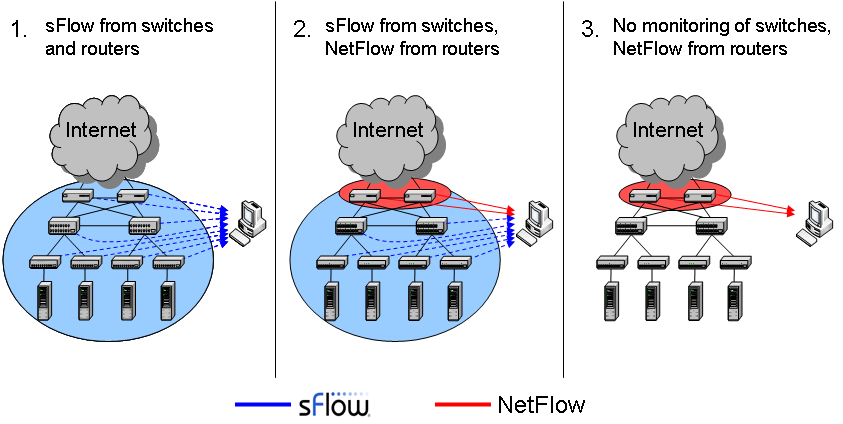
\includegraphics[width=0.8\textwidth]{sflownetflow.PNG}
	\caption[Nasazení NetFlow a sFlow. Zdroj: \cite{flowtechnology}]{Nasazení NetFlow a sFlow. Zdroj: \cite{flowtechnology}}
	\label{img:netflow_sflow}
\end{figure}
Ve třech scénářích je shrnuto typické využití.\cite{flowtechnology}
\begin{enumerate}
	\item Všechny switche a routery podporují sFlow. Data ze switchů a routerů sbírá a vyhodnocuje centrální zařízení, které poskytuje přehled nad všemi zapojenými prvky.
	\item Situace nastává v prostředí, kdy switche podporují sFlow a routery NetFlow. Stává se tak typicky v situacích kdy jsou switche od jiného výrbce než routery. Síťová infrastruktura zůstává celá monitorována.
	\item Switche nepodporují monitorování provozu, routery podporují NetFlow. Monitorování zařízení a provozu je omezen pouze na routery.
\end{enumerate}
\subsubsection{Netflow/IPFIX}
V práci jsou uvedeny informace o NetFlow/IPFIX architektuře, která je podporována kolektorem v systému Nemea. IPFIX je protokol vycházející z NetFlow. NetFlow je protokol vytvořený firmou Cisco Networks, jeho hlavním účelem je monitorování sítě s pomocí toků. IPFIX lze popsat jako kopii NetFlow, která původní NetFlow rozšiřuje o některé důležité parametry.\cite{netflowvsipfix}
Dvě zásadní rozšíření, která přináší IPFIX oproti NetFlow jsou:
\begin{itemize}
	\item IPFIX umožňuje zaznamenávat vendor ID. Tím může výrobce síťového hardwaru přidat své informace do toku. Tento postup umožňuje přenášet v tocích informace, které obvykle zpracovávají monitorovací systémy pomocí SNMP, nebo jsou ukládány do syslogu.
	\item IPFIX oproti NetFlow povoluje proměnnou délku políček
\end{itemize}\par
V obrázku \ref{img:netflow_architecture} je zakresleno základní schéma NetFlow architektury, obsahující exportér, kolektor a analyzér.\par
Exportér je podle IETF popsán jako zařízení (například router) podporující NetFlow služby. Exportér monitoruje pakety vstupující do pozorovaného bodu a z těchto paketů vytváří toky. Informace exportuje v podobě záznamu toku do kolektoru.\par
NetFlow kolektor je popsán jako zařízení, které přijímá záznamy toků z jednoho nebo více exportérů. Obdržené záznamy zpracovává a ukládá informace o záznamu toku. Ukládané záznamy mohou být před uložením ještě agergovány.\cite{ietfnetflow}
Data z kolektoru zpracovává třetí prvek zakreslený v nákresu architektury, analyzer. Analyzer je aplikace, která vyhodnocuje výsledná data, případně vytváří reprezentaci dat pro uživatele.\cite{netflow_arch}
	\begin{figure}[!htbp]\centering
		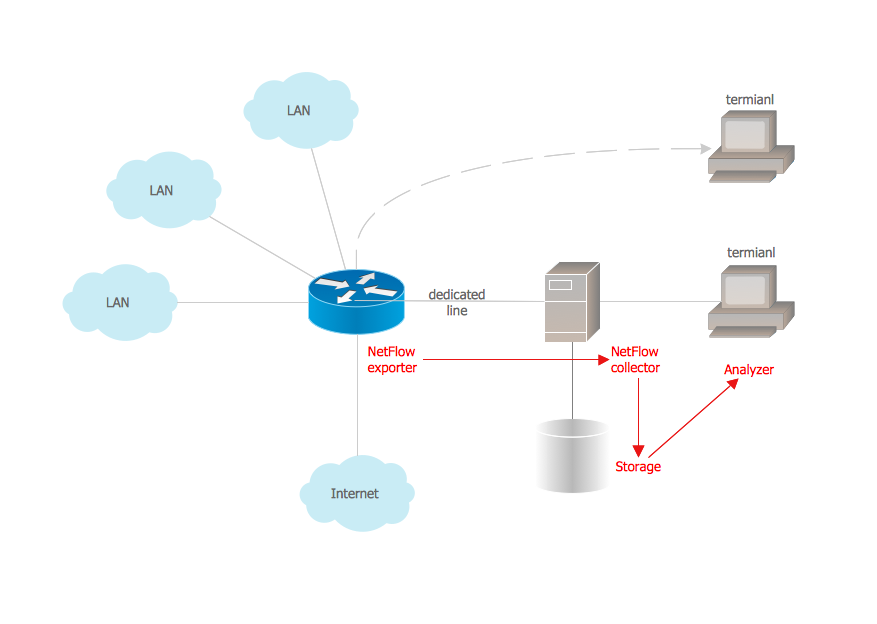
\includegraphics[width=0.8\textwidth]{netflow-architecture.png}
		\caption[Architectura NetFlow. Zdroj: \cite{netflow_arch}]{Architectura NetFlow. Zdroj: \cite{netflow_arch}}
		\label{img:netflow_architecture}
	\end{figure}
\par


\section{Anomálie v síťovém provozu}
Detekce anomálií v síťovém provozu je problémem nalezení neobvyklých vzorů chování v síti, které zasahují mimo hranice síťového provozu, který je určen jako normální.\cite{anomaly} Pro detekování anomálií je potřeba určit referenční stav sítě. Při porovnání s referenčním stavem lze detekovat anomálie. Při vyhodnocování anomálií mohou vznikat falešně pozitivní a falešně negativní stavy. V případě, kdy je nahlášena anomálie, která ve skutečnosti neexistuje, jedná se o falešně pozitivní stav. V případě nenahlášení existující anomálie se jedná o falešně negativní stav. Detekovat anomálie lze s určením konfidenčního intervalu.\newline Konfidenční interval (jinak interval spolehlivosti) lze definovat takto takto:\par
Nechť $ \Theta_{1}$ a $\Theta_{2} $ jsou dvě výběrové statistiky takové, že:
\[ P(\Theta \in (\Theta_{1},\Theta_{2})) = 1 - \alpha \]
kde $\alpha \in (0,1)$. Pak interval $(\Theta_{1},\Theta_{2})$ nazveme intervalem spolehlivosti pro parametr $\Theta$ s parametrem spolehlivosti $1 - \alpha$. Používá se též termínu $100(1 - \alpha)\%$ interval spolehlivosti nebo konfidenční interval.\par
Konfidenční interval je tedy oblast, kde se s určitou pravděpodobností nachází pozorovaný parametr.\cite{confidenceinterval} S tímto mechanizmem lze určovat anomálie s určitou spolehlivostí, na základě toho, jestli se pozorovaný parametr nachází uvnitř nebo mimo konfidenční interval. Toto vyhodnocování vede na statistickou disciplínu testování hypotéz.\cite{hypothesistesting}
Určení konfidenčního intervalu ovlivní citlivost detekce, kdy v případě většího konfidenčního intervalu může docházet k vyššímu množství falešně negativních stavů. Zvolení malého konfidenčního intervalu může naopak vyvolat větší množství falešně pozitivních detekcí.\par 
Ovlivnit spolehlivost detekce lze zvoleným postupem pro detekci anomálie. Jednodušší způsob detekce anomálie je detekovat vždy, když je naměřená hodnota mimo konfidenční interval. Takový způsob detekce může vést na velké množství falešně pozitivních hlášení. Robustnější systém pro detekci je s využitím klouzavého okénka fixní velikosti s řadou výsledků pozorování. Pokud je množství naměřených hodnot překračující konfidenční interval vyšší než předem zvolená hranice, je zaznamenána anomálie.\cite{anomalydetection} Nevýhodou takového řešení je zpoždění v detekci, které odpovídá velikosti klouzavého okénka.
\par Vyhodnocováním různých parametrů sítě lze sledovat změny ve struktuře, v množství síťového provozu, změny rozložení provozu v síti, změny zastoupení různých složek v provozu a dalších vlastností.\par
\subsubsection{Vyhodnocování změn}
Jednou z možností pro sledování a vyhodnocování změn v síti je využití některého generativního síťového modelu, ve kterém je definováno pravděpodobnostní rozdělení pro zkoumané parametry sítě. Jako model může být zvolen některý z generativních modelů pro náhodné grafy(GHRG, stochastický blokový model, hierarchický grafový model, Kroneckerův graf).\cite{graphmodels}\cite{kronecker}\cite{structurechange}\par Tímto způsobem je možné vyhodnocovat změny ve struktuře sítě. Podle vyhodnocování různých parametrů sítě lze pozorovat například:
\begin{itemize}
	\item Rozdělování jedné komunity v síti do dvou.
	\item Spojování dvou komunit do jedné.
	\item Formování komunity, když jedna skupina vytvoří hrany, kterými se spojí s druhou.
	\item Fragmentace, když jedna ze skupin ztratí všechny hrany.
\end{itemize} 
Další možností je změny v síti sledovat na základě vyhodnocování po sobě jdoucích obrazů sítě, rozdělených po časových oknech, kde se jednotlivé obrazy sítě vyhodnocují jako řady skalárních hodnot vyčtených ze sledovaných parametrů sítě. Takto připravené parametry lze zpracovat některou z metod vhodných pro vyhodnocení časových řad.\cite{cumulativestructurechange} Statistické metody jsou podrobněji popsány v kapitole Statistické metody\ref{statistickemetody}. Tímto způsobem je možné monitorovat změny provozu v síti, které mohou ukazovat na probíhající síťové útoky.
Níže jsou uvedeny některé druhy síťových útoků a jejich typické projevy jako síťové anomálie.\ref{dos}\ref{sken}\ref{virus}\ref{botnet}
\subsection{Odmítnutí služby (DOS)}
\label{dos}
Mezi DOS útoky patří více konkrétních druhů útoků. Různé druhy jsou více či méně dobře rozpoznatelné monitorováním toků. Mezi lépe rozpoznatelné patří brute force DOS V tomto typu útoku je podstatou přetížení zdroje nebo sítě, které způsobí nedostupnost služby.\par
Typy DOS útoky obtížně rozeznatelné z analýzy toků jsou založeny na principu sémantického útoku. V těchto případech nedochází k odmítnutí služby na základě zahlcení, ale kvůli obsahu. Příkladem je starší způsob, dnes již známého útkou s názvem Ping of Death. Útočník odesílá záměrně poškozené ping pakety, které způsobí pád systému. Nemožnost identifikace tohoto útoku pomocí toků je způsobena tím, že je při tomto útoku použit pouze jeden ICMP\footnote{Protokol používaný pro oznamování chyb nebo nedostupnosti služby.} tok.
\par...doplnit
\subsection{Skenování}
\label{sken}
\subsection{Viry, červy}
\label{virus}
\subsection{Botnety}
\label{botnet}

\section{Nemea}
\subsection{Struktura systému}
Nemea je framework, který umožňuje sestavení monitorovacího systému z jednotlivých modulů. Moduly komunikují přes vstupní a výstupní rozhraní. Data mezi moduly jsou přenášena pomocí TRAP platformy ve formátu, který specifikuje protokol UniRec. Zpracování dat v Nemea probíhá v reálném čase. Data se posílají jako proudy z výstupních do vstupních rozhraní. Načítání dat je možné provádět v reálném čase z vlastního IPFIX kolektoru nebo číst předem připravená uložená data. V obrázku \ref{img:nemea_example} je zobrazen Nemea systém v konfiguraci pro komplexní monitorování sítě. Aktivní jsou moduly pro sběr dat, zpracování dat, vyhodnocení a detekci anomálií, zpracování a report výsledků.
\begin{figure}[!htbp]\centering
	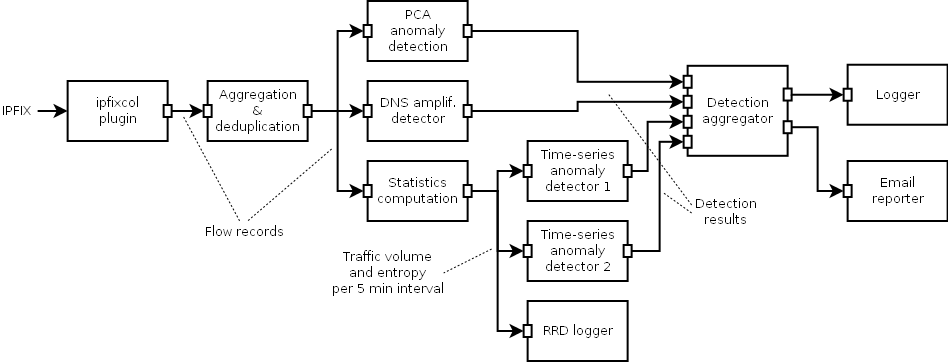
\includegraphics[width=0.9\textwidth]{nemea.png}
	\caption[Příklad Nemea sestavení systému. Zdroj: \cite{nemea}]{Příklad Nemea sestavení systému. Zdroj: \cite{nemea}}
	\label{img:nemea_example}
\end{figure} 
Rozhraní v Nemea jsou implementována jako jednostranná, pro obousměrnou komunikaci tedy musí mít modul definováno minimálně jedno vstupní a jedno výstupní. Formát zasílaných dat je mezi moduly dohodnut při připojení modulu do systému. Modul tak může přijímat a odebírat pouze potřebná data.
\subsection{Moduly}
Každý modul funguje v systému jako samostatný proces. Architektura modulů jako samostatných procesů přináší více možností pro návrh, implementaci a používání modulů, než zpracování systému do jedné zkompilované aplikace.
\begin{itemize}
	\item Moduly mohou být spuštěny a zastaveny v různém čase nezávisle na ostatních.
	\item Moduly lze spravovat ze strany operačního systému nezávisle na dalších částech Nemea systému.
	\item K implementaci modulů je možné použít různé programovací jazyky. 
	\item Zdroje přidělované operačním systémem jsou odděleny pro každý modul (proces).
	\item V případě pádu aplikace se nevyřadí z provozu celý Nemea systém
	\item Moduly lze samostatně aktualizovat.
\end{itemize}
Moduly zachovávají jednotnost ve formátu dat a v použití rozhraní(TRAP,UniRec). Tím si zachovávají kompatibilitu a možnost zapojení do systému. Moduly mohou mít více vstupních i výstupních rozhraní a mohou být spojeny s více moduly. V případě ztráty spojení se pokouší o jeho obnovení. 

\section{Statistické metody}
\label{statistickemetody}
V této sekci jsou popsány metody jednoduchého a exponenciálního klouzavého průměru pro odhadování trendu posloupnosti časových řad, které mohou být využity při vyhodnocování síťového provozu. Dále jsou popsány metody využívající exponenciálního klouzavého průměru pro vícenásobné vyhlazování a predikci hodnot počítajících s trendem a sezónností. S popisem metod je uveden i způsob detekce anomálií.\cite{exponentialsmoothing}
\subsection{Jednoduchý klouzavý průměr}
Metoda jednoduchého klouzavého průměru je založena na výpočtu aritmetického průměru z předchozích období zpracovávané časové řady. Výhodou jednoduchého klouzavého průměru je například oproti exponenciálnímu klouzavému průměru zobrazení skutečného aritmetického průměru z vyhodnocovaných dat.\cite{movingaverages} Vzorec pro výpočet je: 
\[ SMA = \frac{p1 + p2 + \dots + pn}{n} \]
P1 až pn jsou hodnoty z časové řady, n je počet hodnot.

\subsection{Exponenciální vyhlazování}
Exponenciální vyhlazování, jinak exponenciální vyrovnávání, či exponenciální klouzavý průměr, je obdobně jako jednoduchý klouzavý průměr založeno na výpočtu z předchozích pozorovaných hodnot - z časové řady. Oproti jednoduchému klouzavému průměru přináší výhodu v rychlejší reakci na změny při analýze časových řad.\cite{movingaverages}\par Z časové řady je u exponenciálního vyhlazování sestavován trend, který lze vyjádřit jako polynom $k$-tého stupně vzorcem:
\[ \beta_{0} + \beta_{1}t + \beta_{2}t^{2} + \dots + \beta_{k}t^{k} \]
S využitím vzorce trendu lze získat vzorec pro výpočet konkrétní pozorované hodnoty v čase jako:
\[ y_{t-j} = T^{(k)}_{t-j} + \epsilon_{t-j} = \beta_{0} - \beta_{1}j + \beta_{2}j^{2} - \dots + (-1)^{k}\beta_{k}j^{k} + \epsilon_{t-j} \]
kde\newline
$y_{t-j}$ je pozorovaná hodnota,\newline
$t = 1,2,\dots,n$ index aktuální pozice v pozorování,\newline
$j = 0,1,\dots,t-1$ index stáří pozorování vztažený k indexu v okamžiku pozorování,\newline
$\epsilon$ náhodná složka.\newline
Záporné hodnoty ve vzorci jsou z důvodu, že je vzorec odvozován od času $t$, od kterého se další složky odvíjí do minulosti$t-j$.
U exponenciálního vyhlazování jsou přiřazeny k jednotlivým hodnotám ve zpracovávané časové řadě váhy, které směrem do vzdálenější minulosti exponenciálně klesají. Odhad parametrů lze vyjádřit váženou metodou nejmenších čtverců:
\[ \min_{\beta_{0},\dots,\beta{k}}\sum_{j=0}^{t-1}a^{j}(y_{t-j} - T^{(k)}_{t-j})^{2} \]
kde $0 < \alpha < 1$, tudíž $\alpha^{j}$ s rostoucím $j$ klesá. Z tohoto vzorce jsou odvozeny parametry $\beta_{0},\dots,\beta_{k}$. Tímto postupem jsou parametry odvozovány znova z aktuálních dát při každém opakování pozorování. Pro snížení časové náročnosti mohou být využity vyhlazovací statistiky, sestavené z počátečních odhadů parametrů $\beta_{0},\dots,\beta_{k}$, které jsou dále rekurentně aktualizovány.
\subsubsection{Jednoduché exponenciální vyhlazování}
V jednoduchém exponenciálním vyhlazování je trend považován za konstantní:
\[ T_{t-j} = \beta_{0}, j=0,1,\dots,t-1 \]
Hodnoty vyhlazování v čase $t$ jsou vypočteny ze vzorce:
\[ \hat{y}_{t} = (1 - \alpha)y_{t} + \alpha\hat{y}_{t-1}, t = 1,\dots,n \]
Počáteční hodnota $\hat{y}_{0}$ je určena jako aritmetický průměr:
\[ \hat{y}_{0} = \frac{1}{n}\sum_{t = 1}^{n}y_{t} \]
\subsubsection{Dvojité exponenciální vyhlazování}
V metodě dvojitého exponenciální vyhlazování se uvažuje lineární trend:
\[ T_{t - j} = \beta_{0} - \beta_{1}j, j = 0,1,\dots,t - 1 \]
Při výpočtu s využitím vyhlazovacích statistik popsaných v kapitole jednoduchého exponenciálního vyhlazování jsou použity pro výpočet vyhlazovacích statistik tyto vzorce:
\[ S_{t} = (1 - \alpha)y_{t} + \alpha S_{t - 1} \]
\[ S^{[2]}_{t} = (1 - \alpha)S_{t} + \alpha S^{[2]}_{t - 1} \]
Počáteční hodnoty $S_{0}$ a $S^{[2]}_{0}$ jsou získány z odhadnutých parametrů $\beta_{0}(0)$ a $\beta_{1}(0)$:
\[ S_{0} = \hat{\beta}_{0}(0) - \frac{\alpha}{1 - \alpha}\hat{\beta}_{1}(0) \]
\[ S_{0}^{[2]} = \hat{\beta}_{0}(0) - \frac{2\alpha}{1 - \alpha}\hat{\beta}_{1}(0) \]
kde $ \beta_{0}(0) $ a $ \beta_{0}^{[2]}(0) $ jsou spočítány metodou nejmenších čtverců.\par
Vyrovnaná hodnota v čase $ t $ je spočítána vzorcem:
\[ \hat{y}_{t} = 2S_{t} - S^{[2]}_{t} \] 
\subsubsection{Trojité exponenciální vyhlazování}
Trojité exponenciální vyhlazování pracuje s kvadratickým trendem:
\[ T_{t - j} = \beta_{0} - \beta_{1}j + \beta_{2}j^{2}, j = 0,1,\dots,t - 1 \]
Vyrovnávací statistiky lze zapsat rovnicemi:
\[ S_{t} = (1 - \alpha)y_{t} + \alpha S_{t - 1} \]
\[ S^{2}_{t} = (1 - \alpha)S_{t} + \alpha S^{2}_{t - 1} \]
\[ S^{3}_{t} = (1 - \alpha)S^{2}_{t} + \alpha S^{3}_{t - 1} \]
Počáteční hodnoty pro vyhlazovací statistiky jsou vypočítány rovnicemi:
\[ S_{0} = \hat{\beta}_{0}(0) - \frac{\alpha}{1 - \alpha}\hat{\beta}_{1}(0) + \frac{\alpha(1 + \alpha)}{2(1 - \alpha)^2}\hat{\beta}_2(0) \]
\[ S_{0}^{[2]} = \hat{\beta}_{0}(0) - \frac{2\alpha}{1 - \alpha}\hat{\beta}_{1}(0) + \frac{2\alpha(1 + 2\alpha)}{2(1 - \alpha)^2}\hat{\beta}_2(0) \]
\[ S_{0}^{[3]} = \hat{\beta}_{0}(0) - \frac{3\alpha}{1 - \alpha}\hat{\beta}_{1}(0) + \frac{3\alpha(1 + 3\alpha)}{2(1 - \alpha)^2}\hat{\beta}_2(0) \]
$ \beta_{0} $,$ \beta_{1} $,$ \beta_{2} $ jsou získány metodou nejmenších čtverců.\newline
Vyhlazené hodnoty v čase $t$ jsou vypočítány vzorcem:
\[ \hat{y}_t = 3S_{t} - 3S_{t}^{[2]} + 3S_{t}^{[3]} \]

\subsection{Holtova metoda s lineárním trendem}
Holtova metoda exponenciálního vyhlazování trendů (zpracována 1957) pracuje se dvěma vyhlazovacími konstantami $\alpha$ a $\beta$. Konstanta $\alpha$ slouží k adaptivnímu odhadu úrovně $\beta_{0}$ v čase $t$ a $\beta$ pro adaptivní odhad směrnice lineárního trendu $\beta_{1}$ v čase $t$\par
Odhad parametrů $\beta_{0}$ a $\beta_{1}$ v čase $t$ je:
\[ \hat{\beta}_{0,t} = \alpha y_{t} +(1 - \alpha)(\hat{\beta}_{0,t - 1} + \hat{\beta}_{1,t - 1}) \]
\[ \hat{\beta}_{1,t} = \beta(\hat{\beta}_{0,t} - \hat{\beta}_{0,t - 1}) + (1 -\beta)\hat{\beta}_{1,t - 1} \]
kde\newline
$\hat{\beta}_{0,t} $ je odhad úrovně lineárního trendu v čase t, \newline
$\hat{\beta}_{1,t}$ je odhad směrnice lineárního trendu v čase t, \newline
$\hat{\beta}_{0,t - 1}$ je odhad úrovně lineárního trendu v čase $t - 1$,\newline 
$\hat{\beta}_{1,t -1}$ je odhad směrnice lineárního trendu v $t - 1$,\newline 
$\alpha \in <0,1>$ je vyhlazovací konstanta úrovně,\newline 
$\beta \in <0,1>$ je vyhlazovací konstanta směrnice.
Bodová předpověď s horizontem období $h > 0$ v čase $t$ je definována:
\[ \hat{y}_{t}(h) = \hat{\beta}_{0,t} + h\hat{\beta}_{1,t} \]
Pro $h = 1$ v čase $t - 1$ jsou bodová předpověď a chyba předpovědi:
\[ \hat{y}_{t - 1}(1) = \hat{\beta}_{0,t - 1} + \hat{\beta}_{1,t - 1} \]
\[ \hat{a}_{t} = y_{t} - \hat{\beta}_{0,t - 1} - \hat{\beta}_{1,t - 1} \]
\subsection{Holt Wintersova metoda se sezónními trendy}
Winters, Holtův žák, rozšířil Holtovu metodu exponenciálního vyhlazování trendů o aditivní a multiplikativní sezónnost. Metoda využívá třech vyhlazovacích konstant pro hladinu, trend a sezónnost
\par...doplnit
\section{Klasifikace vytížení sítě}
 
\chapter{Návrh}

\section{Struktura navrhnutého modulu}

\chapter{Implementace}
\section{Použité nástoroje}
\section{Součásti modulu}

\chapter{Použití modulu}
\section{Nasazení v systému NEMEA}
\section{Spouštění modulu}

\chapter{Testy}

\begin{conclusion}
	%sem napište závěr Vaší práce
\end{conclusion}

\bibliographystyle{csn690}
\bibliography{mybibliographyfile}

\appendix

\chapter{Seznam použitých zkratek}
% \printglossaries
\begin{description}
	\item[GHRG] Generalized hierarchical random graph
	\item[Nemea] Network measurements analysis
	\item[IDS] Intrusion detection system
	\item[IPFIX] IP Flow Information Export
	\item[TRAP] Traffic analysis platform
	\item[UniRec] Unified record
	\item[SNMP] Simple network management protocol
	\item[ICMP] Internet control message protocol
\end{description}

\chapter{Instalační příručka}

\chapter{Uživatelská příručka}


% % % % % % % % % % % % % % % % % % % % % % % % % % % % 
% % Tuto kapitolu z výsledné práce ODSTRAŇTE.
% % % % % % % % % % % % % % % % % % % % % % % % % % % % 
% 
% \chapter{Návod k~použití této šablony}
% 
% Tento dokument slouží jako základ pro napsání závěrečné práce na Fakultě informačních technologií ČVUT v~Praze.
% 
% \section{Výběr základu}
% 
% Vyberte si šablonu podle druhu práce (bakalářská, diplomová), jazyka (čeština, angličtina) a kódování (ASCII, \mbox{UTF-8}, \mbox{ISO-8859-2} neboli latin2 a nebo \mbox{Windows-1250}). 
% 
% V~české variantě naleznete šablony v~souborech pojmenovaných ve formátu práce\_kódování.tex. Typ může být:
% \begin{description}
% 	\item[BP] bakalářská práce,
% 	\item[DP] diplomová (magisterská) práce.
% \end{description}
% Kódování, ve kterém chcete psát, může být:
% \begin{description}
% 	\item[UTF-8] kódování Unicode,
% 	\item[ISO-8859-2] latin2,
% 	\item[Windows-1250] znaková sada 1250 Windows.
% \end{description}
% V~případě nejistoty ohledně kódování doporučujeme následující postup:
% \begin{enumerate}
% 	\item Otevřete šablony pro kódování UTF-8 v~editoru prostého textu, který chcete pro psaní práce použít -- pokud můžete texty s~diakritikou normálně přečíst, použijte tuto šablonu.
% 	\item V~opačném případě postupujte dále podle toho, jaký operační systém používáte:
% 	\begin{itemize}
% 		\item v~případě Windows použijte šablonu pro kódování \mbox{Windows-1250},
% 		\item jinak zkuste použít šablonu pro kódování \mbox{ISO-8859-2}.
% 	\end{itemize}
% \end{enumerate}
% 
% 
% V~anglické variantě jsou šablony pojmenované podle typu práce, možnosti jsou:
% \begin{description}
% 	\item[bachelors] bakalářská práce,
% 	\item[masters] diplomová (magisterská) práce.
% \end{description}
% 
% \section{Použití šablony}
% 
% Šablona je určena pro zpracování systémem \LaTeXe{}. Text je možné psát v~textovém editoru jako prostý text, lze však také využít specializovaný editor pro \LaTeX{}, např. Kile.
% 
% Pro získání tisknutelného výstupu z~takto vytvořeného souboru použijte příkaz \verb|pdflatex|, kterému předáte cestu k~souboru jako parametr. Vhodný editor pro \LaTeX{} toto udělá za Vás. \verb|pdfcslatex| ani \verb|cslatex| \emph{nebudou} s~těmito šablonami fungovat.
% 
% Více informací o~použití systému \LaTeX{} najdete např. v~\teci{wikilatex}.
% 
% \subsection{Typografie}
% 
% Při psaní dodržujte typografické konvence zvoleného jazyka. České \uv{uvozovky} zapisujte použitím příkazu \verb|\uv|, kterému v~parametru předáte text, jenž má být v~uvozovkách. Anglické otevírací uvozovky se v~\LaTeX{}u zadávají jako dva zpětné apostrofy, uzavírací uvozovky jako dva apostrofy. Často chybně uváděný symbol "{} (palce) nemá s~uvozovkami nic společného.
% 
% Dále je třeba zabránit zalomení řádky mezi některými slovy, v~češtině např. za jednopísmennými předložkami a spojkami (vyjma \uv{a}). To docílíte vložením pružné nezalomitelné mezery -- znakem \texttt{\textasciitilde}. V~tomto případě to není třeba dělat ručně, lze použít program \verb|vlna|.
% 
% Více o~typografii viz \cite{kobltypo}.
% 
% \subsection{Obrázky}
% 
% Pro umožnění vkládání obrázků je vhodné použít balíček \verb|graphicx|, samotné vložení se provede příkazem \verb|\includegraphics|. Takto je možné vkládat obrázky ve formátu PDF, PNG a JPEG jestliže používáte pdf\LaTeX{} nebo ve formátu EPS jestliže používáte \LaTeX{}. Doporučujeme preferovat vektorové obrázky před rastrovými (vyjma fotografií).
% 
% \subsubsection{Získání vhodného formátu}
% 
% Pro získání vektorových formátů PDF nebo EPS z~jiných lze použít některý z~vektorových grafických editorů. Pro převod rastrového obrázku na vektorový lze použít rasterizaci, kterou mnohé editory zvládají (např. Inkscape). Pro konverze lze použít též nástroje pro dávkové zpracování běžně dodávané s~\LaTeX{}em, např. \verb|epstopdf|.
% 
% \subsubsection{Plovoucí prostředí}
% 
% Příkazem \verb|\includegraphics| lze obrázky vkládat přímo, doporučujeme však použít plovoucí prostředí, konkrétně \verb|figure|. Například obrázek \ref{fig:float} byl vložen tímto způsobem. Vůbec přitom nevadí, když je obrázek umístěn jinde, než bylo původně zamýšleno -- je tomu tak hlavně kvůli dodržení typografických konvencí. Namísto vynucování konkrétní pozice obrázku doporučujeme používat odkazování z~textu (dvojice příkazů \verb|\label| a \verb|\ref|).
% 
% \begin{figure}\centering
% 	
\includegraphics[width=0.5\textwidth, angle=30]{cvut-logo-bw}
% 	\caption[Příklad obrázku]{Ukázkový obrázek v~plovoucím prostředí}\label{fig:float}
% \end{figure}
% 
% \subsubsection{Verze obrázků}
% 
% % Gnuplot BW i barevně
% Může se hodit mít více verzí stejného obrázku, např. pro barevný či černobílý tisk a nebo pro prezentaci. S~pomocí některých nástrojů na generování grafiky je to snadné.
% 
% Máte-li například graf vytvořený v programu Gnuplot, můžete jeho černobílou variantu (viz obr. \ref{fig:gnuplot-bw}) vytvořit parametrem \verb|monochrome dashed| příkazu \verb|set term|. Barevnou variantu (viz obr. \ref{fig:gnuplot-col}) vhodnou na prezentace lze vytvořit parametrem \verb|colour solid|.
% 
% \begin{figure}\centering
% 	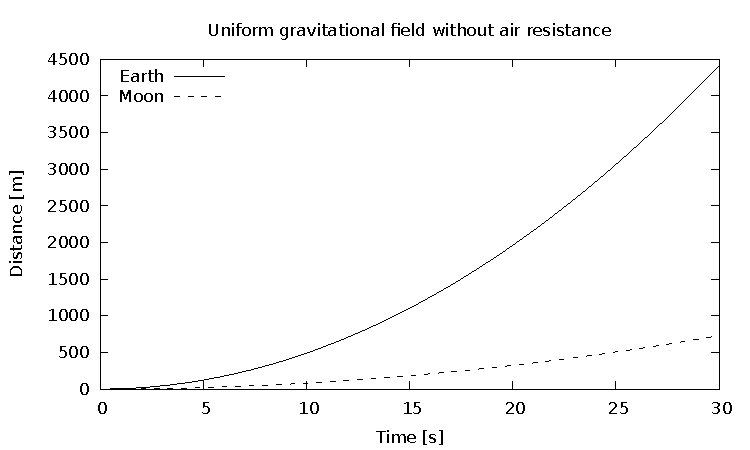
\includegraphics{gnuplot-bw}
% 	\caption{Černobílá varianta obrázku generovaného programem Gnuplot}\label{fig:gnuplot-bw}
% \end{figure}
% 
% \begin{figure}\centering
% 	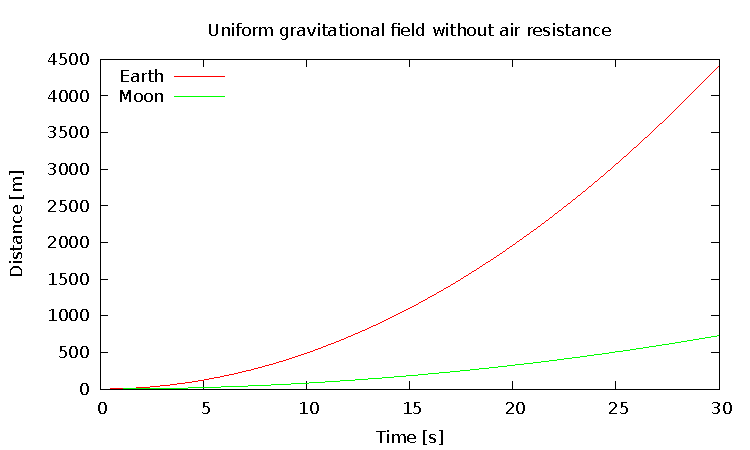
\includegraphics{gnuplot-col}
% 	\caption{Barevná varianta obrázku generovaného programem Gnuplot}\label{fig:gnuplot-col}
% \end{figure}
% 
% 
% \subsection{Tabulky}
% 
% Tabulky lze zadávat různě, např. v~prostředí \verb|tabular|, avšak pro jejich vkládání platí to samé, co pro obrázky -- použijte plovoucí prostředí, v~tomto případě \verb|table|. Například tabulka \ref{tab:matematika} byla vložena tímto způsobem.
% 
% \begin{table}\centering
% 	\caption[Příklad tabulky]{Zadávání matematiky}\label{tab:matematika}
% 	\begin{tabular}{|l|l|c|c|}\hline
% 		Typ		& Prostředí		& \LaTeX{}ovská zkratka	& \TeX{}ovská zkratka	\tabularnewline \hline \hline
% 		Text		& \verb|math|		& \verb|\(...\)|	& \verb|$...$|		\tabularnewline \hline
% 		Displayed	& \verb|displaymath|	& \verb|\[...\]|	& \verb|$$...$$|	\tabularnewline \hline
% 	\end{tabular}
% \end{table}
% 
% % % % % % % % % % % % % % % % % % % % % % % % % % % % 

\chapter{Obsah přiloženého CD}

%upravte podle skutecnosti

\begin{figure}
	\dirtree{%
		.1 readme.txt\DTcomment{stručný popis obsahu CD}.
		.1 exe\DTcomment{adresář se spustitelnou formou implementace}.
		.1 src.
		.2 impl\DTcomment{zdrojové kódy implementace}.
		.2 thesis\DTcomment{zdrojová forma práce ve formátu \LaTeX{}}.
		.1 text\DTcomment{text práce}.
		.2 thesis.pdf\DTcomment{text práce ve formátu PDF}.
		.2 thesis.ps\DTcomment{text práce ve formátu PS}.
	}
\end{figure}

\end{document}
